\documentclass[handout, 10pt]{beamer}

%\usepackage[backend=bibtex,firstinits=true,style=verbose-inote,citestyle=authortitle]{biblatex}
\usepackage{bm}
\usepackage{graphicx}
\usepackage{subcaption}
\usepackage{amsmath}
\usepackage{amsfonts}
\usepackage{makecell}
\usepackage{filecontents}
\usepackage{biblatex}
 \newcommand{\expect}[2][]{
\ifthenelse{\equal{#1}{}}{
\mathbb{E}\left[#2\right]
}{
\underset{#1}{\mathbb{E}}\left[#2\right]
}}

\newcommand{\cov}[2][]{
\ifthenelse{\equal{#1}{}}{
\text{Cov}\left[#2\right]
}{
\underset{#1}{\text{Cov}}\left[#2\right]
}}


\newcommand{\var}[2][]{
\ifthenelse{\equal{#1}{}}{
\text{Var}[#2]
}{
\underset{#1}{\text{Var}}[#2]
}}

\newcommand{\loss}[2][]{
\ifthenelse{\equal{#1}{}}{
\mathcal{L}(#2)
}{
\mathcal{L}_{#1}(#2)
}}

\newcommand{\kl}[2]{
\text{D}_\text{KL}[#1 \parallel #2]
}

\newcommand{\R}{\mathbb{R}}
%\newcommand{\Prob}{\mathbb{P}}

\newcommand{\1}[1]{\mathds{1}\{#1\}}


%\usecolortheme{dolphin}
\setbeamertemplate{navigation symbols}{}
\setbeamertemplate{section in toc}{\inserttocsectionnumber.~\inserttocsection}
\setbeamertemplate{caption}[numbered]

%\begin{filecontents*}{references.bib}
%@misc{FixMatch,
%Author = {Kihyuk Sohn and David Berthelot and Chun-Liang Li and Zizhao Zhang and Nicholas Carlini and Ekin D. Cubuk and Alex Kurakin and Han Zhang and Colin Raffel},
%Title = {FixMatch: Simplifying Semi-Supervised Learning with Consistency and Confidence},
%Year = {2020},
%Eprint = {arXiv:2001.07685},
%}
%\end{filecontents*}
%
%\addbibresource{references.bib}


\title{Latent Generative Memory}
%\subtitle{}
%\author{Ivan Skorokhodov}
%\date{}
%\logo{
\includegraphics[height=1cm]{images/ipavlov-logo.png}}

\newcommand{\citepaper}[1]{\citetitle{#1} by \citeauthor{#1}}

%\graphicspath{{./images}}

%\usetheme{lucid}
\begin{document}

\begin{frame}
    \titlepage
\end{frame}

%\begin{frame}{Our main ideas}
%    Project main ideas are the following:
%    \begin{itemize}
%        \item Propose a continual zero-shot learning method based on creativity loss.
%        \item Propose evaluation strategy
%    \end{itemize}
%\end{frame}

\begin{frame}{Latent Generative Memory (LGM)}
    \pause
    \begin{figure}
        \centering
        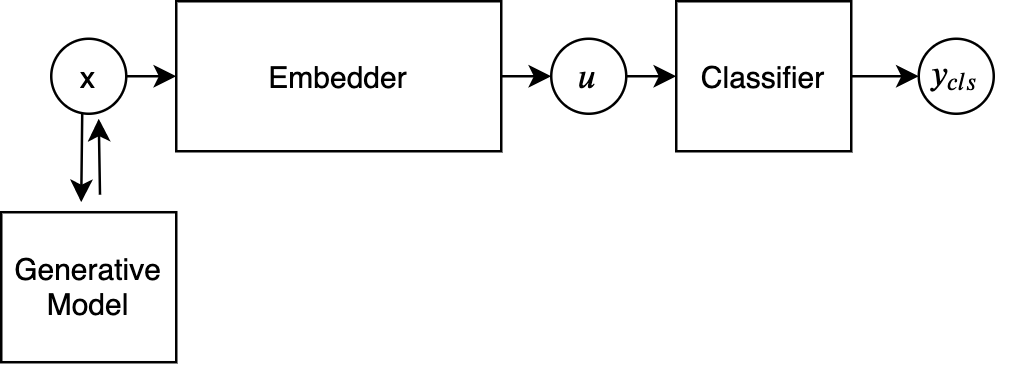
\includegraphics[width=0.6\textwidth]{images/GM}
        \caption{Generative Memory (i.e. a traditional one)}
    \end{figure}
    
    \pause
    \begin{figure}
        \centering
        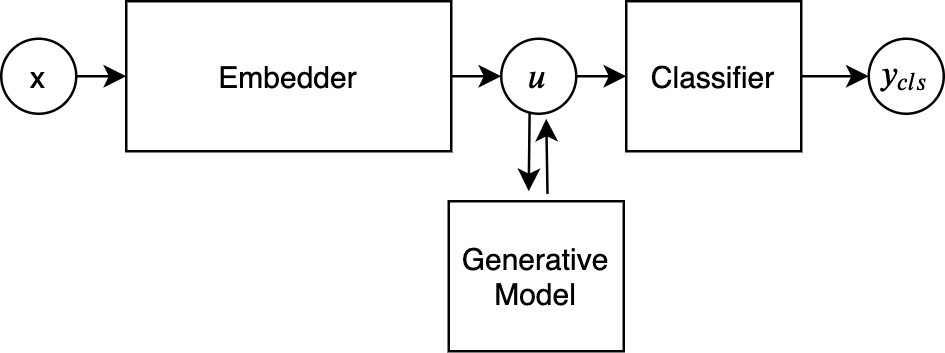
\includegraphics[width=0.6\textwidth]{images/LGM}
        \caption{Latent Generative Memory}
    \end{figure}
    
    \pause
    Remark: one can use any generative model (GAN/VAE/Flows/etc) for their generative memory.
\end{frame}


\begin{frame}{LGM pros and cons}
    \pause Pros:
    \begin{itemize}
        \item\pause Much simpler computationally since training anything in a latent space is easier
        \item\pause Should provide better scores than MeRGAN since huge GANs are difficult to train in an image space, especially continually
    \end{itemize}
    
    \pause Cons:
    \begin{itemize}
        \item\pause It is not obvious how to make Embedder not forget previous data
    \end{itemize}
\end{frame}

\begin{frame}{Making Embedder less forgetful. Strategy \#1.}
\pause Strategy \#1: Apply EWC (or MAS/AGEM/etc.) to Embedder.

\begin{itemize}
    \item\pause Pros: should be easier to implement
    \item\pause Cons:
    \begin{itemize}
        \item\pause It is less novel.
        \item\pause Can work bad in scenarios where EWC (or MAS/AGEM/etc.) work bad. If this is true then things are bad.
    \end{itemize}
\end{itemize}
\end{frame}

\begin{frame}{Making Embedder less forgetful. Strategy \#2.}
\pause Strategy \#2: Apply autoencoding distillation loss:
\begin{itemize}
    \item\pause Train a decoder $D: u \to x$ to decode representations again into images
    \item\pause Apply the following loss:
    \[
    \mathcal{L}^{\text{AE}} = \expect[p^{\text{LGM}}_{t-1}]{\|u - E_t(D_{t-1}(u))\|_2^2}
    \]
    \item\pause Intuition: $\mathcal{L}^{\text{AE}}$ directly forces $E_t$ not to change on previous data.
    \item\pause Pros:
    \begin{itemize}
        \item\pause More novel
        \item\pause Should work well if decoder $D$ is perfect
    \end{itemize}
    
    \item\pause Cons: we are not sure how good our decoder will be
\end{itemize}
\end{frame}

\begin{frame}{LGM-VAE overview}
    Scheme is the same
    \begin{figure}
        \centering
        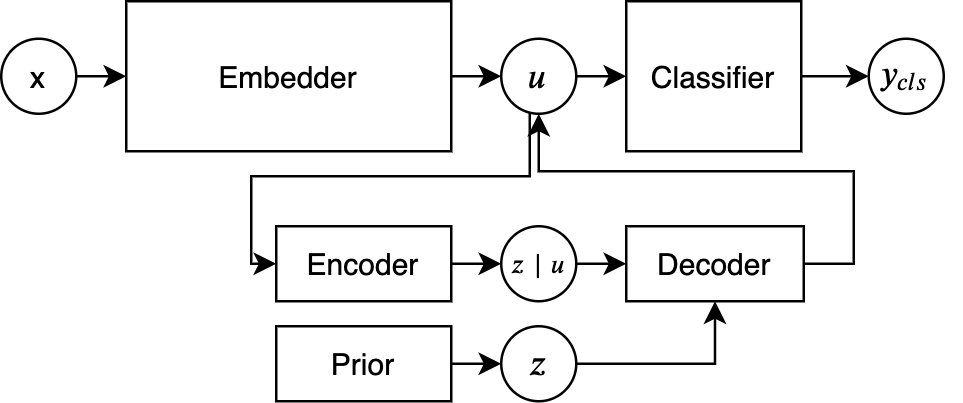
\includegraphics[width=0.6\textwidth]{images/LGM-VAE}
        \caption{VAE-based LGM}
    \end{figure}
    
    \pause
    VAE training specifics:
    \begin{itemize}
        \item\pause We perform distillation for an encoder and a decoder independently:
        \begin{itemize}
            \item For decoder we just sample from prior and optimize $\| D_t(z) - D_{t-1}(z)\|^2$
            \item For encoder we sample $u$ from the previous GM model and optimize $\| E_t(u) - D_{t-1}(u)\|^2$
        \end{itemize}
        \item\pause It should be beneficial to train a prior model to memorize data better
    \end{itemize}
\end{frame}

%\begin{frame}{GM-VAE training}
%    \begin{itemize}
%        \item First, train 
%    \end{itemize}
%\end{frame}

\begin{frame}{LGM-VAE pros and cons}
    Pros:
    \begin{itemize}
        \item training is more stable
        \item gives better scores in preliminary experiments
        \item gives better scores for ``Three scenarios'' paper
    \end{itemize}
    
    Cons:
    \begin{itemize}
        \item Distillation is a bit of ill-posed
        \item GANs should be better at memorizing data?
        \item Not obvious how to force hallucinated samples look real
    \end{itemize}
\end{frame}

\begin{frame}{Continual Learning by Memorization}
    Imagine we have a magic neural network $M$ that:
    \begin{itemize}
        \item\pause Takes a dataset $X$ as an input and memorizes it
        \item\pause Outputs the stored dataset $X$ by demand
        \item\pause Has ``reasonable'' number of parameters (i.e. less than HAT, for example).
    \end{itemize}
    
    We can ``solve'' CL by using $M$:
    \begin{itemize}
        \item\pause For task $1$ store dataset $X_1$ in $M$.
        \item\pause For task $t$ extract all the previous datasets $X_1, ..., X_{t-1}$, concat them and put into $M$
        \item\pause At each timestep $t$ we can extract all the stored data $X_1, ..., X_t$ and train a \textit{joint} classifier (which is an upper bound!).
    \end{itemize}
    
    \pause
    \textbf{Will it be a fair approach?}
\end{frame}

\begin{frame}{Final thoughts}
    \begin{itemize}
        \item\pause ICCV19 model is not an LGM model since they do not use embedder
        \item\pause LGM model, if done properly, seems to be an individual contribution that can be sold individually (i.e. applying a creativity loss can be a separate project after that)
        \item\pause If one is going to build LGM through autoencoding loss than the project is likely to consist on 3 sequential projects:
        \begin{enumerate}
            \item Take any autoencoder, train a generative model in its latent space. How good are the samples?
            \item Put this setup onto continual learning rails, i.e. it allows us to train LGM with autoencoding loss
            \item Apply creativity losses
        \end{enumerate}
        \item\pause ``CL through memorization'' idea can also have potential for two projects:
        \begin{enumerate}
            \item\pause How to build a ``Deep Memorizing Model''?
            \item\pause Show that DMMs solve CL perfectly, implying that there is something wrong with our evaluation of CL.
        \end{enumerate}
    \end{itemize}
\end{frame}

\end{document}
